\chapter{Methods}\label{ch:methods}

\section{Architecture of the Integrated Simulation Environment}\label{sec:architecture-of-the-integrated-simulation-environment}
    The proposed integration consists of the open-source Driving Simulator CARLA\cite{carla2017} and the microscopic traffic simulator TraffSim\cite{backfrieder2013traffsim,backfrieder2014traffsim}, which was developed at the University of Applied Sciences Upper Austria.
    To connect the two simulators into one integrated environment, a gRPC\cite{wang1993grpc} API was added to the microscopic traffic simulator, as well as a REST (Representational State Transfer) Endpoin.
    The gRPC-API is used to transfer data between the simulators during a running Simulation, as well as to transfer control signal (such as: Pausing the Simulation).
    The REST-Endpoint is used by the driving simulator to request the map used for the scenario.
    This map is requested in OpenDrive Format (see Section\ref{sec:road-network-export-and-sync}).

    \subsection{Vehicles in TraffSim}\label{subsec:vehicles-in-traffsim}
        In TraffSim there are a few different Types of Vehicles (see Figure %TODO )

\subsection{Simulation step synchronisation}\label{subsec:simulation-step-synchronisation}
        \begin{figure}
            \centering
            \begin{tikzpicture}
                \node[name=p, shape=pilot, minimum size=1.5cm](uInput){Participant};
                \node[module, right= 2cm of uInput](dSim){CARLA};
                \node[module, right= 2cm of dSim](bridge){Integration bridge};
                \node[module, right= 2cm of bridge](su){SimulationUpdater};
                \node[module, above= 1cm of su](hdvu){VehicleUpdater};
                \node[module, below= 1cm of su](vfm){vehicle-following models};
                \node[fit=(su) (hdvu) (vfm), draw, inner sep=2mm] (tSim){};
                \node[below] at (tSim.south){TraffSim};

                \path[arrowUni] (uInput) to[out=30, in=150] node [text width=2.5cm,midway, above=0.5em,align=center ] {Driver input} (dSim);
                \path [arrowUni] (bridge) to[out=150, in=30] node [text width=2.5cm,midway, above=0.5em,align=center ] {request entity position} (dSim);
                \path [arrowUni] (bridge) to[out=30, in=180] node [text width=2.5cm,midway, above=0.5em,align=center ] {add vehicle update} (hdvu);
                \path [arrowUni] (hdvu) -- node [text width=2.5cm,midway, right=0.5em,align=center ] {} (su);
                \path [arrowUni] (su) to[out=-50, in=50] node [text width=2.5cm,midway, right=0.5em,align=center ] {} (vfm);
                \path [arrowUni] (vfm) to[out=130, in=-130] node [text width=2.5cm,midway, left=0.5em,align=center ] {} (su);
                \path [arrowUni] (su) -- node [text width=2.5cm,midway, left=0.5em,align=center ] {} (bridge);
                \path [arrowUni] (bridge) to[out=-150, in=-30] node [text width=2.5cm,midway, below=0.5em,align=center ] {update entity positions} (dSim);
                \path [arrowUni] (dSim) to[out=-150, in=-30] node [text width=2.5cm,midway, below=0.5em,align=center ] {display} (uInput);
            \end{tikzpicture}
            \caption{Data roundtrip}
            \label{fig:architecture-integration}
        \end{figure}
        The human driver employs the Carla interface to engage with the integrated simulation environment (see Figure\ref{fig:architecture-integration}).
        It is essential that the driving behaviour of the simulation-controlled vehicle appears natural to the human driver.
        Therefore, the time between driver input and the visual output of the driving simulator must be minimised (data round-trip time).
        It is essential that the driver's input is accurately captured by Carla and that the human-driven vehicle is precisely simulated in order to create a realistic driving experience for the driver.
        As the two simulators are not synchronised with regard to their tick rates, the integration bridge requests the current position, speed and acceleration of the vehicle and a vehicle update is added to the update queue of the HumanDrivenVehicleUpdater within the traffic simulator.
        Upon calculation of the subsequent simulation step in the traffic simulator, all vehicle updates that have been queued are executed, thereby updating the human-driven vehicle.
        Therefore, the delta time between simulation steps should be selected as low as possible, in order to minimise the data round-trip time.


    \subsection{Real time simulation}\label{subsec:real-time-simulation}
        %FIXME: redo
        although $t$ must not be lower than the time it takes for the simulation step to be calculated $T$.
        To bind the simulation time to the real time, the easiest way would be to set the time step size to the time duration it took for the last simulation step to compute:
        \[
            t_{x} = T_{x-1}
        \]
        The problem with that approach is, that during a simulation in TraffSim it should be avoided to change the simulation step $t$, so another approach is used, by adding a delay after each simulation step to compensate for the difference between $t$ and $T$.
        It`s important for this technique to work, the condition $t \geq T$ has to be met.
        In every simulation step the added delay $d$ has to be calculated and thus $t$ can be static:
        \[
            d_{x} = t - T_x
        \]

\section{TraffSim API}\label{sec:traffsim-api}
    To interact with the microscopic traffic simulator TraffSim, a gRpc\cite{wang1993grpc} API was specified and developed, which allows the client to call the functions described in Listing\ref{lst:traffSim-api-proto}.
    The Api was designed to allow the client to control all the functions that are important during a simulation session and also to sync the two simulators.



\begin{GenericCode}[caption={TraffSim API proto}, label={lst:traffSim-api-proto}]
service TraffSimController {
    rpc requestVehicleData (ActiveSimulationRun)
        returns (VehicleData);
    rpc notifyFreeDrivingVehicle(FreeDrivingVehicleUpdateRequest)
        returns(VoidMessage){}
    rpc simulationAllowTswConnection (ActiveSimulationRun)
        returns (BoolMessage) {}
    rpc getAvailableFreeDrivingVehicles(ActiveSimulationRun)
        returns(AvailableFreeDrivingVehicles){}
    rpc getAvailableScenarios (VoidMessage)
        returns (AvailableScenarios){}
    rpc getOpenSimulations (VoidMessage)
        returns (ActiveSimulationRuns){}
    rpc getSimulationState (ActiveSimulationRun)
        returns (SimulationState){}
    rpc pauseSimulation (ActiveSimulationRun)
        returns (VoidMessage){}
    rpc startSimulation (ActiveSimulationRun)
        returns (VoidMessage){}
    rpc setSimulationResolution (SimulationResolutionRequest)
        returns (VoidMessage){}
    rpc setSimulationDelay (SimulationDelayRequest)
        returns (VoidMessage){}
}\end{GenericCode}

\section{Mapped dummy vehicles}\label{sec:mapped-dummy-vehicles}
    In TraffSim, there are several different types of vehicles (see Figure ).%TODO:class diagram
    The human-driven vehicles are able to traverse the entire map and are not constrained to the road network, whereas the simulation-controlled vehicles are constrained to the road network.

    In order for the vehicle-following models to react to the human driver, it is necessary to represent the human-driven vehicle on the "rail-like" road network.
    Dummy vehicles are placed on the road network at each time step to enable the model-controlled vehicles to interact with the human-controlled vehicle.
    A map-matching algorithm is employed to identify the locations where dummy vehicles should be placed.

    \subsection{Map matching}\label{subsec:map-matching}
        To determine the position, a dummy vehicle has to be placed on the road network, a map-matching algorithm is used.

\section{Speed and Acceleration projection}\label{sec:speed-and-acceleration-projection}
    In order to allow the vehicle-following models to work, the human driven vehicle`s speed $\vec{v_h}$ and acceleration $\vec{a_h}$ need to be mapped onto the dummy vehicle.
    Therefore $\vec{a_h}$ and $\vec{v_h}$ are projected onto the tangent vector of the nearest road segment $\vec{R}$.
    Since a mapped vehicle is bound to the road network and thus traveling "on rails", the speed and acceleration can be expressed as scalars ($a_m$ and $v_m$), which act like the magnitude of the speed vector in the direction of the current Road segment.
    The idea behind this mapping is to allow model-controlled vehicles to react to human-controlled vehicles, even if they are not traversing the road network as expected.
    To achieve the desired behavior some cases have to be considered, the cases described below can be seen in Figure\ref{fig:vehicleTravelingCases} :

    \begin{encase}
        \item Vehicle driving on the nearest road.
        In this case the speed and acceleration vector of the mapped vehicle should be equal to the speed and acceleration of the human-controlled vehicle.
        \begin{align*}
            \vec{v_h} \times \vec{R} = 0 &\Rightarrow v_m = |\vec{v_h}| \\
            \vec{a_h} \times \vec{R} = 0 &\Rightarrow a_m = |\vec{a_h}|
        \end{align*}

        \item Vehicle crossing the nearest road.
        In the case of a vehicle crossing the nearest road, the speed of the mapped vehicle should be zero.
        This is used to block the road for upcoming vehicles when one such human-controlled crosses the road.
        \begin{align*}
            \vec{v_h} \cdot \vec{R} = 0 &\Rightarrow v_m = 0 \\
            \vec{a_h} \cdot \vec{R} = 0 &\Rightarrow a_m = 0
        \end{align*}
        \item Vehicle moving on the road on an angle.
        Like in the 2 cases before the speed and acceleration of the mapped vehicle should correspond to the component of the speed and acceleration vector of the human-controlled vehicle (see Figure\ref{fig:vehicleTravelingCases})
        In this case the angle between the road and the vehicles speed and acceleration vectors has to be calculated.
        \[
            \cos(\phi_{h,\vec{R}}) = \frac{\vec{v_h} \cdot  \vec{R}}{|\vec{v_h}| |\vec{R}|}
        \]
    \end{encase}

    To combine all the cases above the speed and acceleration are projected onto $\vec{R}$:

    \begin{align*}
        v_m = |\vec{v_h}| * \cos(\phi_{h,\vec{R}}) &= \frac{\vec{v_h} \cdot \vec{R}}{|\vec{R}|}\\
        a_m = |\vec{a_h}| * \cos(\phi_{h,\vec{R}}) &= \frac{\vec{a_h} \cdot \vec{R}}{|\vec{R}|}
    \end{align*}


    \begin{figure}
        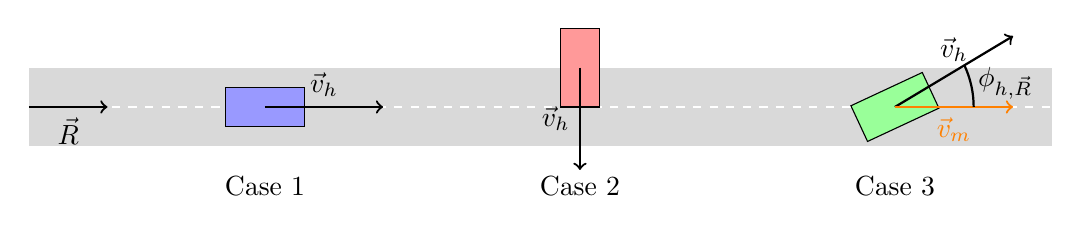
\begin{tikzpicture}

            % Draw the road as a gray rectangle
            \fill[gray!30] (-7,-0.5) rectangle (6,0.5);

            % Draw the center line of the road
            \draw[dashed, white, thick] (-7,0) -- (6,0);

            % Case 1: Vehicle driving on the road (aligned)
            \node[draw, fill=blue!40, minimum width=1cm, minimum height=0.5cm] (vehicle1) at (-4, 0) {};
            \node at (-4, -1) {Case 1};
            \draw[->, thick] (-4, 0) -- (-2.5, 0) node[midway, above] {$\vec{v}_h$};

            % Case 2: Vehicle crossing the road (perpendicular)
            \node[draw, fill=red!40, minimum width=1cm, minimum height=0.5cm, rotate=90] (vehicle2) at (0, 0.5) {};
            \node at (0, -1) {Case 2};
            \draw[->, thick] (0, 0.5) -- (0, -0.8) node[midway, left] {$\vec{v}_h$};

            % Case 3: Vehicle moving at an angle to the road
            \node[draw, fill=green!40, minimum width=1cm, minimum height=0.5cm, rotate=25] (vehicle3) at (4, 0) {};
            \node at (4, -1) {Case 3};
            \draw[->, thick] (4, 0) -- (5.5, 0.9) node[midway, above] {$\vec{v}_h$};

            % Draw the projection onto the road for Case 3
            \draw[dotted, thick] (4, 0) -- (4.5, 0);
            \draw[->, thick, orange] (4, 0) -- (5.5, 0) node[midway, below] {$\vec{v}_m$};

            % Draw the angle phi for Case 3
            \draw[thick] (5, 0) arc (0:25:1.25);
            \node at (5.4, 0.3) {$\phi_{h,\vec{R}}$};

            % Draw the road vector R
            \draw[->, thick] (-7, 0) -- (-6, 0) node[midway, below] {$\vec{R}$};
        \end{tikzpicture}
        \caption{Cases of vehicles traveling on road network}
        \label{fig:vehicleTravelingCases}
    \end{figure}




\section{Road network export and sync}\label{sec:road-network-export-and-sync}


